\begin{enumerate}
	\item \textbf{Register}
	
	Registering a Voter collects all the data required for a user to be valid and adds that information to the Voter database. Once the Voter has been added to the database they will have access to a minimum system. The minimum system only allows them to log in and view where they can go to get activated (to allow access to the entire system) to allow them to participate in the current election.
	
		\begin{enumerate}
			\item \textbf{Service Contract}
				\begin{figure}[H]
					\centering
					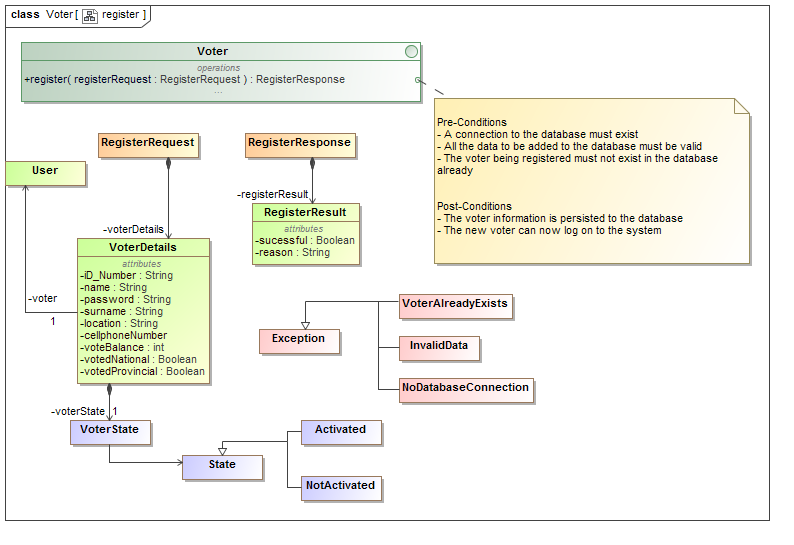
\includegraphics[width=0.75\linewidth]{../Images/Voter/ServiceContracts/register_serviceContract.png}
					\caption{Register Voter Service Contract}
				\end{figure}
				
			Register creates an initial state for a Voter and captures all the provided information in the database. Once information has been added to the database, the user can edit it themselves by accessing their account once they have logged in. Only valid data will be accepted. 
				\newline				
				
				\begin{enumerate}
					\item Pre-conditions
					\begin{itemize}
						\item There must be a connection to the database
						\item The information provided by the user must be valid.
						\item The user must not exist in the current database. 
					\end{itemize}
					
					\item Exceptions
					\begin{itemize}
						\item If there is no connection to the database, the NoDatabaseConnection exception will be thrown.
						\item If the data is invalid then the service is refused and the InvalidData exception is thrown.
						\item If the user already exists in the database then the service is refused and the UserAlreadyExists exception is thrown.
					\end{itemize}
					
					\item Post-conditions
					\begin{itemize}
						\item The new Voter can log in and access the Electronic Voting system. 
						\item The Voter’s information is persisted to the database.
					\end{itemize}
				\end{enumerate}
			
			\item \textbf{Functional Requirements}
				\begin{figure}[H]
					\centering
					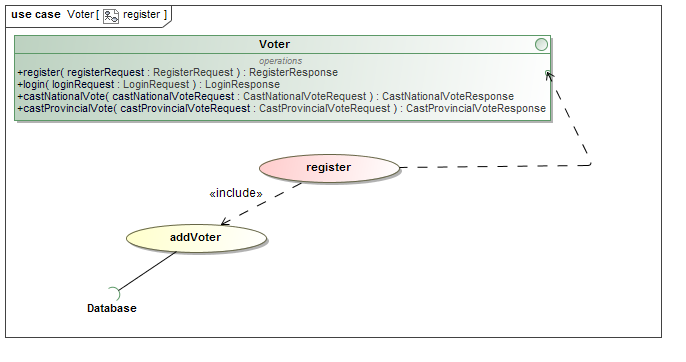
\includegraphics[width=0.75\linewidth]{../Images/Voter/UseCases/register_useCase.png}
					\caption{Register Voter Use-Case}
				\end{figure}
				
				\begin{enumerate}
					\item The registerRequest object encapsulates all the necessary information required to add a new Voter to the system. 
					\item All the information collected by the register function is persisted to the database through the Database module's addVoter function. 
				\end{enumerate}
				
			
			
			
			\item \textbf{Process Design}
				\begin{figure}[H]
					\centering
					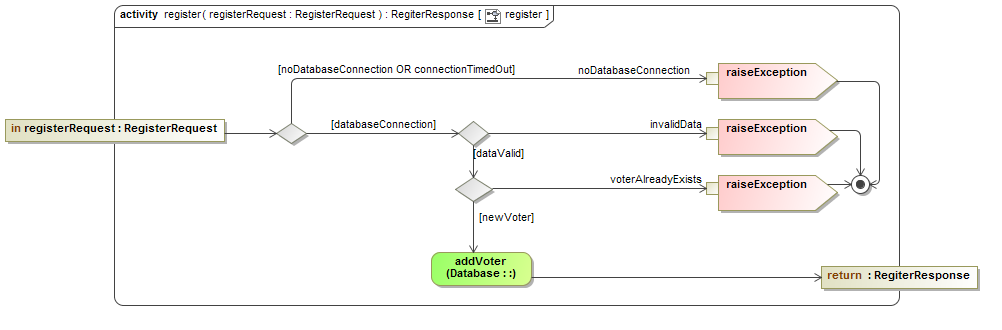
\includegraphics[width=0.75\linewidth]{../Images/Voter/ActivityDiagrams/register_activity.png}
					\caption{Register Voter Activity}
				\end{figure}
				
				\begin{enumerate}
					\item The Register function first checks to see if there is a connection to the database, if there is not or the connection times out, the NoDatabaseConnection exception is thrown. 
					\item If there is a database connection, it checks whether the Voter's data is valid(according to the data types specified in the database). 
					\item If the data is not valid, the InvalidData exception is thrown. 
					\item Then the function checks whether the Voter's information already exists in the database and throws the VoterAlreadyExists exception if the Voter already exists.
					\item Otherwise no exception is thrown and the Voter's information is persisted to the database using the Database module's addVoter function. 
					
				\end{enumerate}
				
				
\end{enumerate}
	
	\item \textbf{Login}
	
	Login functionality gives the user access to system and allows them to view their account information, and only once they have been activated, are they allowed to cast votes and view other relevant information. 
	
		\begin{enumerate}
			\item \textbf{Service Contract}
			\begin{figure}[H]
				\centering
				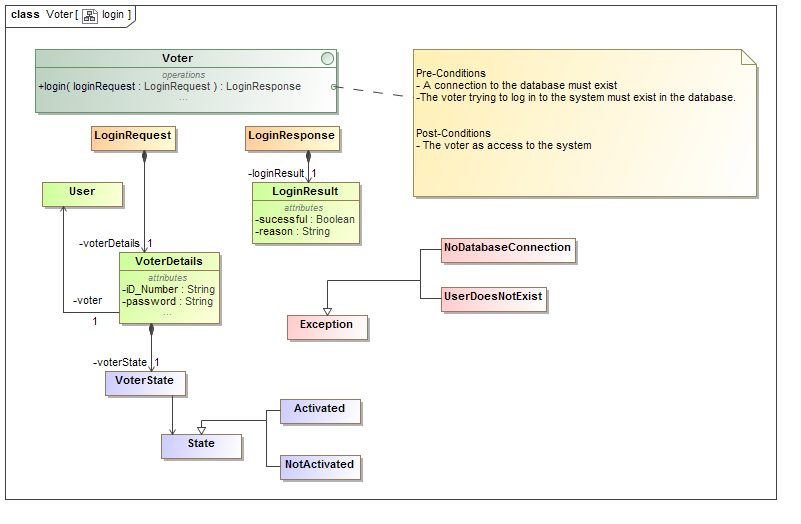
\includegraphics[width=0.75\linewidth]{../Images/Voter/ServiceContracts/login_serviceContract.png}
				\caption{Login Service Contract}
			\end{figure}
			
			Login validates a user and gives them rights to interact with the core system. 
			\newline
			
			\begin{enumerate}
				\item Pre-conditions
				\begin{itemize}
					\item There must be a connection to the database
					\item The user must have already registered. 
				\end{itemize}
				
				\item Exceptions
				\begin{itemize}
						\item If there is no connection to the database, the NoDatabaseConnection exception will be thrown
						\item If the user has not registered then the UserDoesNotExist exception is thrown and the service is denied. 
				\end{itemize}
				
				\item Post-conditions
				\begin{itemize}
					\item The Voter has access to the Electronic Voting system.
				\end{itemize}
			\end{enumerate}
			
			\newpage
			
			\item \textbf{Functional Requirements}
			\begin{figure}[H]
				\centering
				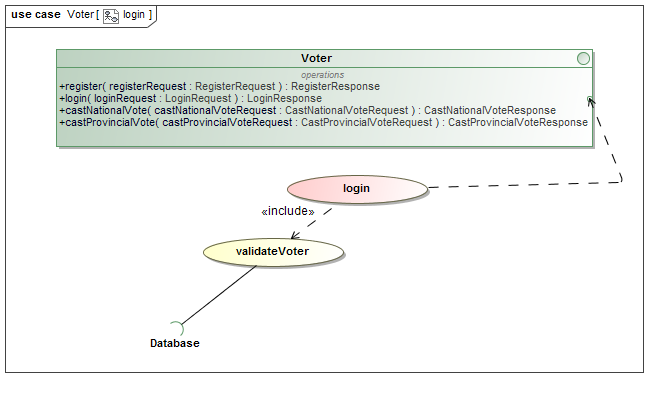
\includegraphics[width=0.75\linewidth]{../Images/Voter/UseCases/login_useCase.png}
				\caption{Login Voter Use-Case}
			\end{figure}
			
			\begin{enumerate}
				\item The login use-case collects Voter information which will be used to validate a Voter. 
				\item A Voter is invalid if their credentials do not checkout. 
				\item The Voter module's login passes information to the Database modules validateVoter function to check whether the Voter attempting to log in is valid or not.  
			\end{enumerate}
			
			\item \textbf{Process Design}
			\begin{figure}[H]
				\centering
				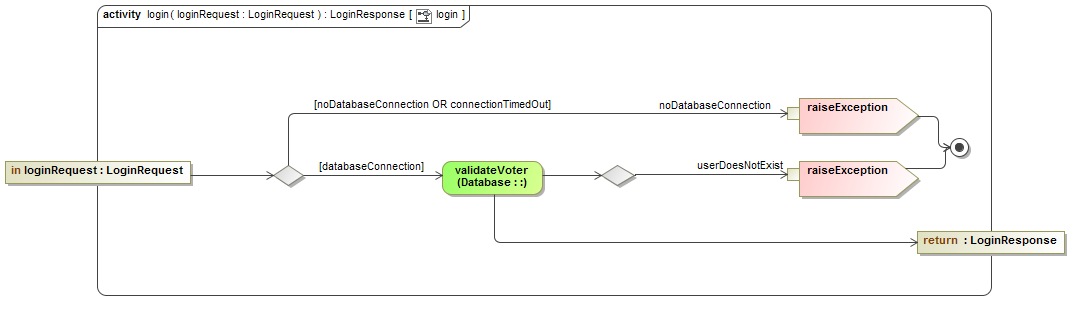
\includegraphics[width=0.75\linewidth]{../Images/Voter/ActivityDiagrams/login_activity.png}
				\caption{Login Voter Activity}
			\end{figure}
			
			
			\begin{enumerate}
				\item The Login function first checks to see if there is a connection to the database, if there is not or the connection times out, the NoDatabaseConnection exception is thrown.
				\item Then it calls the Database module's validateUser function which will return an object that contains a boolean value of whether the voter is valid (and can thus access the system) as well as a reason or false (thus the Voter is denied access) as well as reason as to why the service has been denied. 
				\item The UserDoesNotExist exception is thrown if validateUser returns false. 
			\end{enumerate}			
		\end{enumerate}

\newpage

	\item \textbf{Cast National Vote}
	
	Casting a vote requires voter to be logged in.
	
	\begin{enumerate}
		\item \textbf{Service Contract}
		\begin{figure}[H]
			\centering
			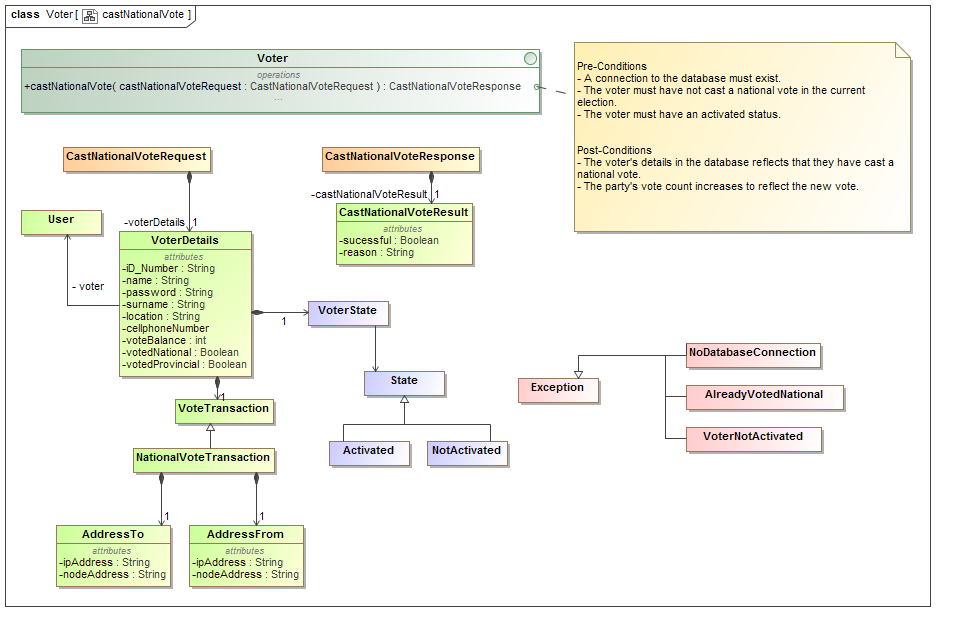
\includegraphics[width=0.75\linewidth]{../Images/Voter/ServiceContracts/castNationalVote_serviceContract.png}
			\caption{Cast National Vote Service Contract}
		\end{figure}
		
		Once the Voter is logged in we can retrieve their account information to view their location and their current vote balance(calculated by whether they have voted national, provincial or neither). \newline
	 The voting node’s address for the current voter(based on the user’s location) as well as the party node’s address are retrieved, this information will be sent to the Blockchain Module to concretely cast the voters vote as Blockchain transaction.
		\newline				
		
		\begin{enumerate}
			\item Pre-conditions
			\begin{itemize}
				\item There must be a connection to the database
				\item The Voter must not have already cast a National vote in the current election. 
				\item The Voter must have an Activated status.  
			\end{itemize}
			
			\item Exceptions
			\begin{itemize}
				\item If there is no connection to the database, the NoDatabaseConnection exception will be thrown.
				\item If the Voter has already cast a National vote, the AlreadyVotedNational exception is thrown and the service is denied.
				\item If the Voter has not been activated by an Activator, the VoterNotActivated exception is thrown and they are disallowed from casting a vote. 
			\end{itemize}
			
			\newpage
			
			\item Post-conditions
			\begin{itemize}
				\item Voter details in the database reflect that they have cast a National Vote. 
				\item The Party which the Voter has voted for shows an increment by one in their node balance. 
			\end{itemize}
		\end{enumerate}
		
		\item \textbf{Functional Requirements}
		\begin{figure}[H]
			\centering
			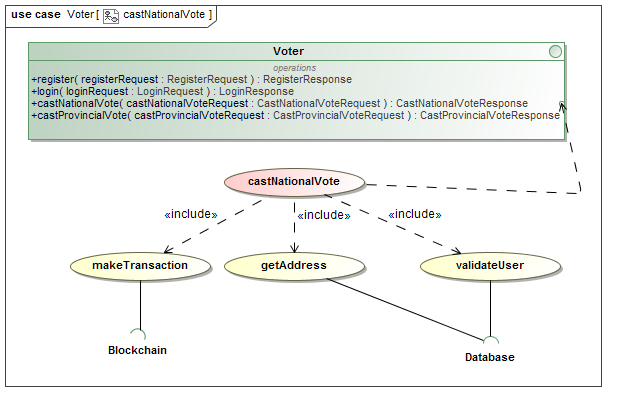
\includegraphics[width=0.75\linewidth]{../Images/Voter/UseCases/castNationalVote_useCase.png}
			\caption{Cast National Vote Use Case}
		\end{figure}
		
		\begin{enumerate}
			\item The Cast National Vote use case starts uses the database to retrieve the addresses of the Party which is being voted for as well as the Voting region node's addresses.   
			\item Once it has all the addresses, it uses the Blockchain's makeTransaction functionality to cast the vote into the Blockchain. (Sending one coin from the Voting Region Node to the coin accepting Party Node of the Voter's choice.) 
		\end{enumerate}
		
		\item \textbf{Process Design}
		\begin{figure}[H]
			\centering
			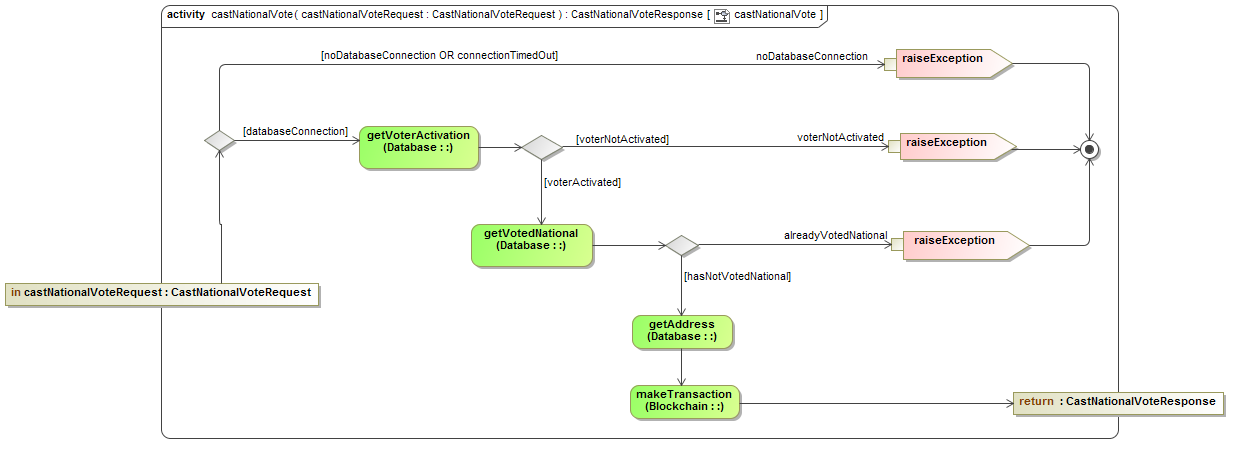
\includegraphics[width=0.75\linewidth]{../Images/Voter/ActivityDiagrams/castNationalVote_activity.png}
			\caption{Cast National Vote Activity}
		\end{figure}
		
		\begin{enumerate}
			\item The function first checks to see if there is a connection to the database, if there is not or the connection times out, the NoDatabaseConnection exception is thrown. 
			\item If a connection exists, it proceeds to check whether the Voter has been activated or not. 
			\item If the Voter has not been activated, the VoterNotActivated exception is thrown. 
			\item Then the function checks whether the Voter has already cast a National vote. If they have the AlreadyVotedNational exception is thrown.
			\item If none of the exceptions are thrown, the function then queries the database to find all of the necessary addresses then it calls the Blockchain's makeTransaction function to cast the actual vote.  
			
		\end{enumerate}
	\end{enumerate}

	\item \textbf{Cast Provincial Vote}
	
	Casting a vote requires voter to be logged in.
	
	\begin{enumerate}
		\item \textbf{Service Contract}
		\begin{figure}[H]
			\centering
			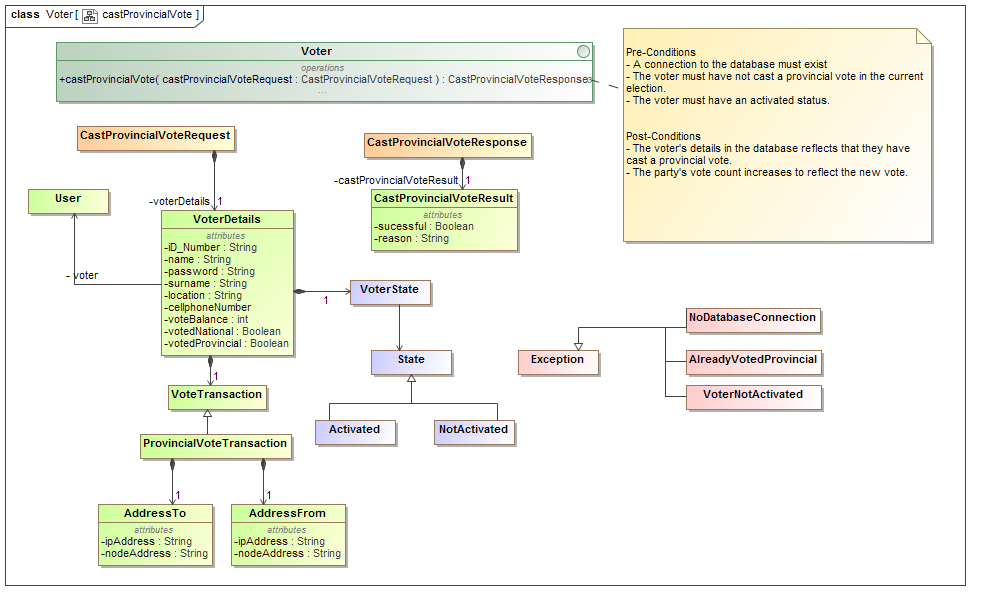
\includegraphics[width=0.75\linewidth]{../Images/Voter/ServiceContracts/castProvincialVote_serviceContract.png}
			\caption{Cast Provincial Vote Service Contract}
		\end{figure}
		
		Once the Voter is logged in we can retrieve their account information to view their location and their current vote balance(calculated by whether they have voted national, provincial or neither). \newline
		The voting node’s address for the current voter(based on the user’s location) as well as the party node’s address are retrieved, this information will be sent to the Blockchain Module to concretely cast the voters vote as Blockchain transaction.
		\newline				
		
		\begin{enumerate}
			\item Pre-conditions
			\begin{itemize}
				\item There must be a connection to the database
				\item The Voter must not have already cast a Provincial vote in the current election. 
				\item The Voter must have an Activated status.  
			\end{itemize}
			
			\item Exceptions
			\begin{itemize}
				\item If there is no connection to the database, the NoDatabaseConnection exception will be thrown.
				\item If the Voter has already cast a National vote, the AlreadyVotedProvincial exception is thrown and the service is denied.
				\item If the Voter has not been activated by an Activator, the VoterNotActivated exception is thrown and they are disallowed from casting a vote. 
			\end{itemize}
			
			\item Post-conditions
			\begin{itemize}
				\item Voter details in the database reflect that they have cast a Provincial Vote. 
				\item The Party which the Voter has voted for shows an increment by one in their node balance. 
			\end{itemize}
		\end{enumerate}
		
		\item \textbf{Functional Requirements}
		\begin{figure}[H]
			\centering
			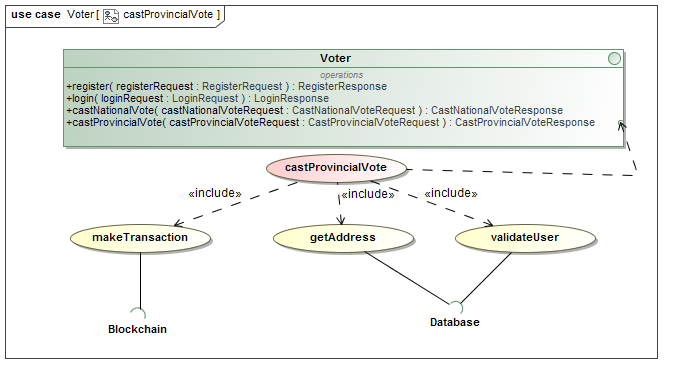
\includegraphics[width=0.75\linewidth]{../Images/Voter/UseCases/castProvincialVote_useCase.png}
			\caption{Cast Provincial Vote Use Case}
		\end{figure}
		
		\begin{enumerate}
			\item The Cast Provincial Vote use case starts uses the database to retrieve the addresses of the Party which is being voted for as well as the Voting region node's addresses.   
			\item Once it has all the addresses, it uses the Blockchain's makeTransaction functionality to cast the vote into the Blockchain. (Sending one coin from the Voting Region Node to the coin accepting Party Node of the Voter's choice.) 
		\end{enumerate}
		
		\newpage
		
		\item \textbf{Process Design}
		\begin{figure}[H]
			\centering
			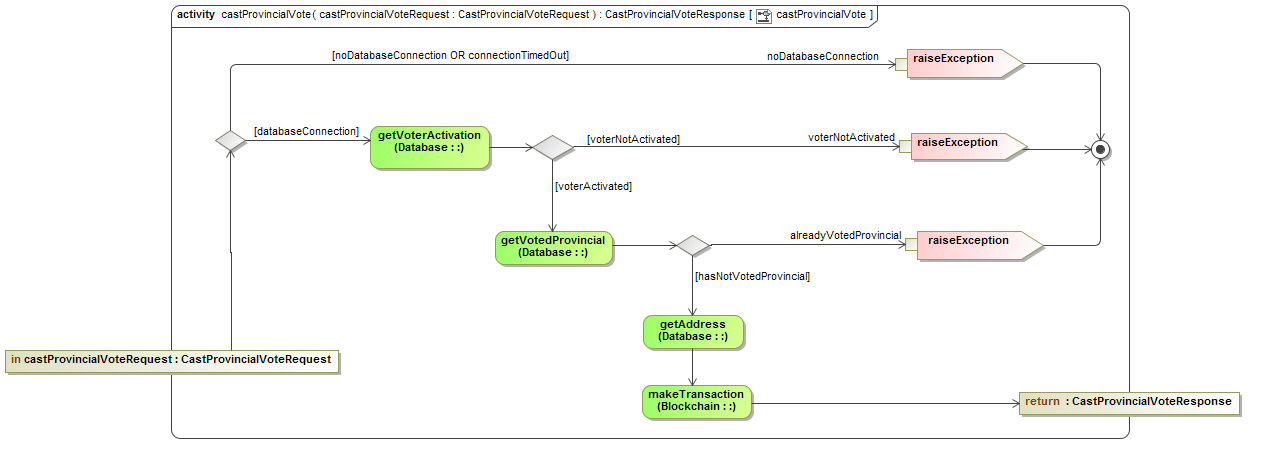
\includegraphics[width=0.75\linewidth]{../Images/Voter/ActivityDiagrams/castProvincialVote_activity.png}
			\caption{Cast Provincial Vote Activity}
		\end{figure}
		
		\begin{enumerate}
			\item The function first checks to see if there is a connection to the database, if there is not or the connection times out, the NoDatabaseConnection exception is thrown. 
			\item If a connection exists, it proceeds to check whether the Voter has been activated or not. 
			\item If the Voter has not been activated, the VoterNotActivated exception is thrown. 
			\item Then the function checks whether the Voter has already cast a Provincial vote. If they have the AlreadyVotedProvincial exception is thrown.
			\item If none of the exceptions are thrown, the function then queries the database to find all of the necessary addresses then it calls the Blockchain's makeTransaction function to cast the actual vote.  
			
		\end{enumerate}
	\end{enumerate}
\end{enumerate}









